% This is the file named 'GroupSound.tex'
% @LaTeX-file{
% author = {Matthew Corley and William DeMeo},
% filename = {'GroupSound.tex'}
% date = {2014/01/08},
% text = {main documentation file for the GroupSound project}
% }

%%%% DOCUMENTCLASS %%%%%%%%%%%%%%%%%%%%%%%%%%%%%%%%%%%%%%%%%%%%%%
\documentclass[reqno,onecolumn,oneside]{paper}

%%%% PACKAGES %%%%%%%%%%%%%%%%%%%%%%%%%%%%%%%%%%%%%%%%%%%%%%%
\usepackage{latexsym,amscd,amsmath,amssymb,amsthm,stmaryrd,mathrsfs,enumerate,scalefnt}
\usepackage{tikz}
\usepackage{color}
\usetikzlibrary{calc}
\usepackage[colorlinks=true,urlcolor=black,linkcolor=black,citecolor=black]{hyperref}
\usepackage[printonlyused,smaller]{acronym}
%%%%%%%%%%%%%%%%%%%%%%%%%%%%%%%%%%%%%%%%%%%%%%%

%%%% MACROS %%%%%%%%%%%%%%%%%%%%%%%%%%%%%%%%%%%%%%
\newcommand{\lb}{\ensuremath{\llbracket}}
\renewcommand{\rb}{\ensuremath{\rrbracket}}
\newcommand{\<}{\ensuremath{\langle}}
\renewcommand{\>}{\ensuremath{\rangle}}
\newcommand{\sdp}{\ensuremath{\rtimes}}
\newcommand{\inverse}[1]{\ensuremath{#1^{-1}}}
\newcommand{\zmv}{\ensuremath{x^m k_v}}
\newcommand{\zmvInv}{\ensuremath{x^{N-wm} k_w}}

   \newcommand{\field}[1]{\ensuremath{\mathbb{#1}}}
   \newcommand{\N}{\field{N}}                   % natural numbers
   \newcommand{\Z}{\field{Z}}                   % integers
   \newcommand{\Q}{\field{Q}}                   % rationals
   \newcommand{\R}{\field{R}}                   % reals
   \newcommand{\Rn}{\ensuremath{\field{R}^n}}                % the set of n-tuples with elements in \R
   \newcommand{\C}{\field{C}}                   % complex numbers 
   \newcommand{\Cn}{\ensuremath{\field{C}^n}}                % the set of n-tuples with elements in \C


   \newcommand{\vs}[1]{\ensuremath{\mathcal{#1}}}
   \newcommand\sL{\vs{L}}
   \newcommand{\LA}{\vs{L}(A)}        % the collection of complex valued functions of $A$.
   \newcommand{\LG}{\vs{L}(G)}        % the collection of complex valued functions of $G$.
   \newcommand{\LZn}{\vs{L}(\Z/n\Z)}    % the collection of complex valued functions of $\Z/N$.

   % LINEAR TRANSFORMATIONS: use sansserif with \lt,as in \lt{T}.
   \newcommand{\lt}[1]{\ensuremath{\mathsf{#1}}}
   \newcommand{\T}{\lt{T}}       % a linear operator (\eg translation)
   \newcommand\conv{\lt{C}}

   % VECTORS: use bold font
   \newcommand\vf{\ensuremath{\mathbf{f}}}

   % GROUP ALGEBRA
   \newcommand{\ga}[1]{\ensuremath{\C #1}} %  group algebras
   \newcommand{\CA}{\ga{A}}                % the group algebra of $A$
   \newcommand{\CG}{\ga{G}}                % the group algebra of $G$


\newcommand{\defn}[1]{\emph{#1}}

%%%% To add notes about things that need to be fixed/addressed, use todo
     \newcommand{\todo}[1]{
     {\bf TODO(wjd):} \emph{#1}\\
     }

%%%% TITLE/AUTHOR/DATE %%%%%%%%%%%%%%%%%%%%%%%%%%%%%%%
\title{What does a nonabelian group sound like?}
\subtitle{Harmonic Analysis on Finite Groups and DSP Applications}
\author{Matthew Corley and William DeMeo}
\institution{University of South Carolina}

%%%% END PREAMBLE %%%%%%%%%%%%%%%%%%%%%%%%%%%%%%%



\begin{document}

\maketitle

%--ABSTRACT---------------------------------------------------------------------------
\begin{abstract}
Underlying many \ac{dsp} algorithms, in particular those used for digital audio
filters, is the convolution operation, which is a weighted sum of translations
$f(x-y)$. Most classical results of \ac{dsp} are easily and elegantly derived if
we define our functions on $\Z/n\Z$, the abelian group of integers modulo $n$. 
If we replace this underlying ``index set'' with a nonabelian group, then
translation may be written $f(y^{-1}x)$, and the resulting audio filters arising
from convolution naturally produce different effects that those obtained with
ordinary (abelian group) convolution. 

The goal of this project is to explore the idea of using the underlying finite
group (i.e., the index set) as an adjustable parameter of a digital audio
filter. By listening to samples produced using various nonabelian groups, we try
to get a sense of the ``acoustical characters'' of finite groups.
\end{abstract}


%=======================================================================
%--INTRO----------------------------------------------------------------
\section{Introduction}
The \emph{translation-invariance} of most classical signal
processing transforms and filtering operations is largely
responsible for their widespread use, and is crucial for
efficient algorithmic implementation and interpretation 
of results~\cite{An:2003}. 

\ac{dsp} on \emph{finite abelian groups} such as $\Z/n\Z$ is
well understood and has great practical utility.  
Translations are defined using addition modulo $n$, and 
basic operations, including convolutions and Fourier 
expansions, are developed relative to these translations~\cite{Tolimieri:1998}. 
Recently, however, interest in the practical utility of
\emph{finite nonabelian groups} has grown
significantly. Although the theoretical foundations of
nonabelian groups is well established, application of the
theory to \ac{dsp} has yet to  become common-place.
A notable exception is~\cite{An:2003},
which develops theory and algorithms for
indexing data with nonabelian groups, defining translations
with a non-commutative group multiply operation, and
performing typical \ac{dsp} operations relative to these
translations. 

This paper describes the use of nonabelian groups
for indexing one- and two-dimensional signals, and discusses 
some computational advantages and insights that can be gained from 
such an approach. 
A simple but instructive class of 
nonabelian groups 
is examined.  When elements of such
groups are used to index the data, and standard \ac{dsp}
operations are defined with respect to special group
binary operators, more general and interesting
signal transformations are possible.
\subsection{Preview: Two Distinctions of Consequence}
Abelian group \ac{dsp} can be completely described in terms of a
special class of signals called the \emph{characters} of the
group. (For $\Z/n\Z$, the characters are simply the exponentials.)
Each character of an abelian group represents a one-dimensional
translation-invariant subspace, and the set of all characters
spans the space of signals indexed by the group; any such
signal can be uniquely expanded as a linear combination over
the characters.

In contrast, the characters of a nonabelian group $G$
do not determine a basis for the space of signals indexed by
$G$.  However, a basis can be constructed by extending the
characters of an abelian subgroup $A$ of $G$, and then taking
certain translations of these extensions.  Some of the
characters of $A$ cannot be extended to characters of $G$,
but only to proper subgroups of $G$.  This presents some
difficulties involving the underlying translation-invariant
subspaces, some of which are now multidimensional.
However, it also presents opportunities for alternative
views of local signal domain information on these
translation-invariant subspaces. 

The other abelian/nonabelian distinction of primary importance 
concerns translations defined on the group.  In the abelian group
case, translations represent simple linear shifts in space or time.
When nonabelian groups index the data, however, translations are no
longer so narrowly defined. 

\subsection{Brief overview of nonabelian convolution}
Since the main operation we will consider is convolution, we must 
think about how best to view this operation mathematically, as well as how best to
represent it in the computer.  In this section is some background on the
mathematical aspects.  In later sections we provide more details and examples.

Let $\C^G$ denote the set of complex valued functions defined on the group
$G$.  That is 
\[
\C^G = \{f : G\rightarrow \C \}.
\]
(In the Tolimieri-An books, \cite{Tolimieri:1998} \cite{Tolimieri:2003}, this set is also denoted by
$\sL(G)$.)  If the group has $|G| = n$ elements, say, 
$G = \{x_0, x_1, \dots, x_{n-1}\}$, 
then each function $f\in  \C^G$ can be represented as
a length-$n$ vector in $\C^n$---namely, the vector of its values on $G$:
\[
\vf = [f(x_0), f(x_1), \dots, f(x_{n-1})].
\]

Given two functions $f$ and $g$ in $\C^G$, the \emph{convolution of
$f$ and $g$}, denoted, $f*g$, is also function in $\C^G$ and is
defined by the values it takes at each $x\in G$ as follows:
\begin{equation}
\label{eq:1}  
(f*g)(x) = \sum_{y \in G} f(y) g(y^{-1}x).
\end{equation}
Note that this is a weighted sum of translations of $g$.
Indeed, let $\T_y: \C^G\rightarrow \C^G$ denote
the \emph{translation by $y$} operator---that is, $\T_y$ maps 
a function $g\in \C^G$ to a translated version of itself, $\T_y(g)$, which is defined at each 
$x \in G$ by $\T_y(g)(x) = g(y^{-1}x)$.
Then~(\ref{eq:1}) can be written as
\begin{equation}
\label{eq:4}  
(f*g)(x) = \sum_{y \in G} f(y) \T_y(g)(x),
\end{equation}
a sum of weighted translations of $g$ where 
the coefficients $f(y)$ are the weights, and 
$\T_y(g)$ is the function $g$ ``shifted'' by $y$. (When $G$ is the abelian
group $\Z/n\Z$ with addition modulo $n$, we have
$\T_y(g)(x) = g(y^{-1}x) = g(x-y)$, so in this case
$\T_y(g)$ is literally $g$ shifted by $y$ units to the right.)

Equation~(\ref{eq:4}) defines the convolution, $f * g$, by giving its
value at each $x\in G$. Using the 
translation operator, however, we can define convolution
 ``functionally,'' instead of element-wise, as follows:
\begin{equation}
\label{eq:2}  
f*g = \sum_{y \in G} f(y) \T_y(g)
\end{equation}
(Pause to look at the right hand side of~(\ref{eq:2}), and let it sink in that
this is a function that takes arguments $x\in G$; compare with the right
hand side of~(\ref{eq:4}).)

 This is fine, but it is also useful to think of~(\ref{eq:2}) as $f$ acting
on $g$.  Indeed, on the right hand side of~(\ref{eq:2}) we have the operator 
$\sum_{y \in G} f(y) \T_y$ that maps the function $g$ to the function $f*g$.  But
on the left hand side we have a binary operation $f*g$, written in infix
notation, which doesn't jibe very well with this functional interpretation.  So,
instead of saying ``the convolution of $f$ and $g$'', and writing $f*g$, we will
say
%% \emph{convolution by $f$ of $g$} 
``the convolution {\bf by} $f$ {\bf of} $g$,'' and write $\conv(f)(g)$. In this
way, we have the \emph{convolution by $f$} operator:
\begin{equation}
\label{eq:3}  
\conv(f) = \sum_{y \in G} f(y) \T_y,
\end{equation}
which is a weighted sum of translation operators.  The function $\conv(f)$ takes other
functions, like $g$, as its argument.

So, the functional types we have here are the following:
\[
\conv : \C^G \rightarrow (\C^G)^{\C^G}
\]
Given $f\in \C^G$,
\[
\conv(f) : \C^G \rightarrow \C^G
\]
Given $f\in \C^G$ and $g\in \C^G$,
\[
\conv(f)(g) : G \rightarrow \C
\]
Or, in the notational style of a functional programming language like Scala:
\[
\conv : (G \Rightarrow \C) \Rightarrow ( (G \Rightarrow \C) \Rightarrow (G \Rightarrow \C) )
\]
Given $f\in \C^G$,
\[
\conv(f) : (G \Rightarrow \C) \Rightarrow (G \Rightarrow \C)
\]
Given $f\in \C^G$ and $g\in \C^G$,
\[
\conv(f)(g) : (G \Rightarrow \C)
\]


%--CYCLIC---------------------------------------------------------------------------
%============================================================
\section{Background: Finite Groups}
%============================================================
\label{sec:hafg}
\todo{Decide whether this section should go in the appendix.}

This section summarizes the notations, definitions, and important facts needed
below. The presentation style is terse since the goal of this section is to
distill from the more general literature only those results that are most
relevant to our application. 
The books~\cite{An:2003} and~\cite{Tolimieri:1998} treat similar material in a
more thorough and rigorous manner. Throughout, $\C$ denotes complex numbers, 
$G$ an arbitrary finite group, and $\LG$ the collection of complex valued
functions defined on $G$. Other notations for $\LG$ are $\C^G$ and 
$\{f : G \rightarrow \C\}$.

\subsection{Cyclic Groups}
A group $C$ is called a \emph{cyclic group} if there exists $x\in C$ such that
every $y\in C$ has the form $y=x^n$ for some integer $n$.  In this case, we call
$x$ a \emph{generator} of $C$, and we say that such a group is \emph{one generated}.

If $G$ is an arbitrary finite group, and $x\in G$, then the set of powers of $x$,
\begin{equation}
  \label{eq:cyclic-group}
\<x\> = \{x^n : n\in \Z\},
\end{equation}
is a cyclic subgroup of $G$ called the 
\emph{group generated by} $x$ \emph{in} $G$.

It will be convenient to have notation for a cyclic group of
order $N$ without reference to a particular underlying group.
Let the set of formal symbols
\begin{equation}\label{eq:cyclicGroup}
C_N(x) = \{ x^n : 0 \leq n < N\}
\end{equation} 
denote the cyclic group of order $N$ with
generator $x$, and define binary composition by
\begin{equation}\label{eq:binarycomp}
x^m x^n = x^{m+n}, \quad 0\leq m, n < N,
\end{equation}
where $m+n$ is addition modulo $N$.  Then $C_N(x)$ is a
cyclic group of order $N$ having generator $x$. The identity
element of $C_N(x)$ is $x^0 = 1$, and the inverse of $x^n$
in $C_N(x)$ is $x^{N-n}$.

To say that a group is \emph{abelian} is to specify that the binary
composition of the group is commutative, in which case the
symbol $+$ is usually used to represent this operation.
For nonabelian groups, we write the (non-commutative) binary
composition as multiplication.  Since our work involves
both abelian and nonabelian groups, it is notationally
cleaner to write the binary operations of an arbitrary group --
abelian or otherwise -- as multiplication. The
following examples illustrate that additive groups, such as $\Z/N\Z$, have
simple multiplicative representations. 

\begin{example}
{\bf Example.} Let $\Z_N = \{0, 1, \ldots, N-1\}$,
and let addition modulo $N$ be the binary composition defined on $\Z_N$.
This group is isomorphic to the cyclic group $C_N(x)$, 
\[
\Z_N = \{ n : 0 \leq n < N\} \simeq \{ x^n : 0 \leq n < N\}
= C_N(x),
\]
and it is by this identification that the binary composition
of $\Z_N$ can be written as multiplication. 
More precisely, by uniquely identifying each element $m \in \Z_N$
with the corresponding element $x^m \in C_N(x)$, the binary composition
$m+n$ is replaced with that of~(\ref{eq:binarycomp}).  
\end{example}


\begin{example}
{\bf Example.} For an integer $\ell \in \Z_N$, denote by 
$\<x^\ell\>$ 
the subgroup generated by $x^\ell$ in $C_N(x)$. If $\ell$ divides $N$,
then   
\[
%gp_N(x^L) 
\<x^\ell\> = \{x^{m\ell} : 0\leq m < M\}, \quad \ell M = N,
\]
and $\<x^\ell\>$ is a cyclic group of order $M$.
\end{example}

%---
\subsection{Group of Units}
%---
Multiplication modulo $N$ is a ring product on the group of
integers $\Z_N$. An element $m\in \Z_N$ is called a {\it unit} if
there exists an $n\in \Z_N$ such that $mn = 1$.  The set
$U(N)$ of all units in $\Z_N$ is a group with respect to
multiplication modulo $N$, and is called the 
\emph{group of units}.%unit group} of $\Z/N\Z$. 
The group of units can be described %characterized 
as the set of all integers $0<m<N$ such that $m$ and $N$ are
relatively prime.  
\begin{example}
For $N=8$, 
%\begin{equation}\label{eq:unitGroup}
$U(8) = \{1, 3, 5, 7\}$.
%\end{equation}
\end{example}

%======================================================================
%--TRANS---------------------------------------------------------------
\section{Translation Invariance}
%======================================================================
%-----------------------------------------------------------------------
\subsection{Generalized Translation and Convolution}
%-----------------------------------------------------------------------
%\ismasubsubsec{General definition of translation}
For $y\in G$, the mapping $\lt{T}_y$ of $\LG$ defined by 
\begin{equation}\label{eq:trans}
(\lt{T}_yf)(x) = f(y^{-1}x), \quad x \in G,
\end{equation}
is a linear operator of $\LG$ called 
\emph{left translation by} $y$.

%---
%\ismasubsubsec{General definition of convolution}
%---
The mapping $\lt{C}(f)$ of $\LG$ defined by 
\begin{equation}
\lt{C}(f) = \sum_{y\in G} f(y) \lt{T}_y, \quad f\in \LG,
\end{equation}
is a linear operator of $\LG$ called 
\emph{left convolution by} $f$.  By definition, for $x\in G$,
\begin{equation}\label{eq:conv}
(\lt{C}(f)g)(x) = \sum_{y\in G} f(y) g(y^{-1}x), \quad g \in \LG.
\end{equation}
%The collection of all left convolutions of $\LG$ is
%$\vs{C}(G) = \left\{\lt{C}(f) : f \in G \right\}$.

For $f, g \in \LG$, the composition
$f * g  = \lt{C}(f)g$
is called the \emph{convolution product}.
The vector space $\LG$ paired with the convolution product
is an algebra, the \emph{convolution algebra over} $G$.

To gain some familiarity with the general 
definitions of translation %~(\ref{eq:trans}) 
and convolution, %~(\ref{eq:conv}), 
it helps to verify 
that these definitions agree with what we expect 
when $G$ is a familiar abelian group. 
%---
\begin{example}
{\bf Example:}
If $G=\Z_N$, then~(\ref{eq:trans}) becomes
\begin{equation}
(\lt{T}_yf)(x) = f(x-y),  \qquad x \in G,
\end{equation}
and~(\ref{eq:conv}) becomes
\begin{equation}
(\lt{C}(g)f)(x) =\sum_{y \in G} g(y)f(x-y).
\end{equation}
\end{example}

%--GA---------------------------------------------------------------------------
% 
%-----------------------------------------------------------------------
\subsection{The Group Algebra $\CG$}
%-----------------------------------------------------------------------
\label{sec:groupalgebra}
The \emph{group algebra} $\CG$ is the space of all formal sums
\begin{equation}
f = \sum_{x\in G} f(x) x, \quad f(x) \in \C,
\end{equation}
with the following operations for $f, g \in \CG$:
\begin{equation}
f+g = \sum_{x\in G} (f(x) + g(x))x,
\end{equation}
\begin{equation}
\alpha f = \sum_{x\in G} (\alpha f(x)) x, 
           \quad \alpha \in \C,
\end{equation}
\begin{equation}
fg = \sum_{x\in G}\left(\sum_{y\in G} f(y)g(y^{-1}x)\right)x. 
\end{equation}

The mapping $\lt{L}(g)$ of $\CG$ defined by 
$\lt{L}(g)f = gf$
is a linear operator on the space $\CG$ called 
\emph{left multiplication by} $g$.  
Since $y\in G$ can be identified with the formal
sum $e_y \in \CG$ consisting of a single nonzero term,
\begin{equation}\label{eq:leftmult}
yf = \lt{L}(e_y)f = \sum_{x\in G}f(y^{-1}x) x.
\end{equation}
In relation to translation of $\LG$, (\ref{eq:leftmult}) is the
$\CG$ analog. Fig.~\ref{fig:cyclicshift} illustrates.

The mapping $\Theta: \LG \to \CG$ defined by
\begin{equation}\label{eq:iso}
\Theta(f) = \sum_{x\in G} f(x) x, \quad f\in \LG,
\end{equation}
is an algebra isomorphism of the convolution algebra $\LG$
onto the group algebra $\CG$.  
Thus we can identify
$\Theta(f)$ with $f$, using  context to decide whether
$f$ refers to the function in $\LG$ or the formal sum in
$\CG$.  

An important aspect of the foregoing isomorphism is the
correspondence between the translations of the spaces.
Translation of $\LG$ by $y\in G$ %$\T(y)$ 
corresponds to left multiplication of $\CG$ by $y\in G$.
%$\lt{L}(y)$ 
Convolution of $\LG$ by $f\in \LG$ corresponds to
left multiplication of $\CG$ by $f\in \CG$. 
%We state 
%these relations symbolically as follows:
%\begin{center}
%\begin{tabular}{ccc}
%  $\LG$ & $\simeq$ & $\CG$ \\
%  $\lt{T}(y)$ & $\leftrightarrow$ & $\lt{L}(y)$\\
%  $\lt{C}(f)$ & $\leftrightarrow$ & $\lt{L}(f)$
%\end{tabular}
%\end{center}

\begin{figure}
\centerline{\framebox{
	\includegraphics[width=\columnwidth]{t_cyclicshift}}}
  \caption{An impulse $f\in \CA$ and a few abelian group translates, $x^2f, x^9f,
      x^{-7}f$.}
  \label{fig:cyclicshift}
\end{figure}

%\begin{figure}
%%  \centerline{\epsfig{figure=figures/t_cyclicshift,width=70mm, height=50mm}}
%  \centering
%\includegraphics[width=80mm, height=70mm]{t_cyclicshift}
%  \caption{An impulse $f\in \CA$ and a few abelian group translates, $x^2f, x^9f,
%      x^{-7}f$.}
%  \label{fig:cyclicshift}
%\end{figure}

%------------------------------------------------------------------------
\subsection{Ideals: Translation-Invariant Subspaces}
%------------------------------------------------------------------------
A subspace $\vs{V}$ of the space $\CG$ is called a
\emph{left ideal} if 
\begin{equation}
u\vs{V} = \{uf : f \in \vs{V}\} \subset \vs{V}, \quad u \in G. 
\end{equation}
A left ideal of $\CG$ corresponds to a subspace of $\LG$
invariant under all left translations.  

If $\vs{V}$ is a left ideal, then, by linearity, 
$g\vs{V} \subset \vs{V}$ for all $g \in \CG$.
The set $\CG g$, defined by 
$\{fg : f \in \CG\}$, is a left ideal of $\CG$,
called \emph{the left ideal generated by} $g$ in $\CG$. 
%$\CG g = \CG$ if and only if $g$ is an invertible element in $\CG$. 
A left ideal $\vs{V}$ of $\CG$ is called \emph{irreducible}
if the only left ideals of $\CG$ contained in $\vs{V}$ are
$\{0\}$ and $\vs{V}$. The sum of two distinct, irreducible
left ideals is always a direct sum. 
% (\cite{An:2003}, p.~129).

For \emph{abelian} group $A$, the group algebra $\C A$ of
signals is decomposed into a direct sum of irreducible ideals.  
Since multiplication of $\C A$ by elements of $A$
corresponds to translation, ideals represent
translation-invariant subspaces.  Furthermore, in the 
abelian case, such translation-invariant subspaces are
one-dimensional.   

Similarly, for \emph{nonabelian} group $G$, the group algebra
$\CG$ is decomposed into a direct sum of left ideals. Here,
again, the ideals are translation-invariant 
subspaces.  However, some of these subspaces must now be
multi-dimensional, and herein lies the potential advantage
of using nonabelian groups for indexing the data. The left
translations are more general and represent a broader class of 
transformations. Therefore, projections of data into the
resulting left ideals can reveal more complicated partitions
and structures in the data as compared with the Fourier
components in the abelian group case. 

%-----------------------------------------------------------------------
\subsection{The Group Algebra $\CG$}
%-----------------------------------------------------------------------
\label{sec:groupalgebra}
The \emph{group algebra} $\CG$ is the space of all formal sums
\begin{equation}
f = \sum_{x\in G} f(x) x, \quad f(x) \in \C,
\end{equation}
with the following operations for $f, g \in \CG$:
\begin{equation}
f+g = \sum_{x\in G} (f(x) + g(x))x,
\end{equation}
\begin{equation}
\alpha f = \sum_{x\in G} (\alpha f(x)) x, 
           \quad \alpha \in \C,
\end{equation}
\begin{equation}
fg = \sum_{x\in G}\left(\sum_{y\in G} f(y)g(y^{-1}x)\right)x. 
\end{equation}

The mapping $\lt{L}_g$ of $\CG$ defined by 
$\lt{L}_gf = gf$
is a linear operator on the space $\CG$ called 
\emph{left multiplication by} $g$.  
Since $y\in G$ can be identified with the formal
sum $e_y \in \CG$ consisting of a single nonzero term,
\begin{equation}\label{eq:leftmult}
yf = \lt{L}_{e_y}f = \sum_{x\in G}f(y^{-1}x) x.
\end{equation}
In relation to translation of $\LG$, (\ref{eq:leftmult}) is the
$\CG$ analog. Fig.~\ref{fig:cyclicshift} illustrates.

The mapping $\Theta: \LG \to \CG$ defined by
\begin{equation}\label{eq:iso}
\Theta(f) = \sum_{x\in G} f(x) x, \quad f\in \LG,
\end{equation}
is an algebra isomorphism of the convolution algebra $\LG$
onto the group algebra $\CG$.  
Thus we can identify
$\Theta(f)$ with $f$, using  context to decide whether
$f$ refers to the function in $\LG$ or the formal sum in
$\CG$.  

An important aspect of the foregoing isomorphism is the
correspondence between the translations of the spaces.
Translation of $\LG$ by $y\in G$ %$\T(y)$ 
corresponds to left multiplication of $\CG$ by $y\in G$.
Convolution of $\LG$ by $f\in \LG$ corresponds to
left multiplication of $\CG$ by $f\in \CG$. 
We state 
these relations symbolically as follows:
\begin{center}
\begin{tabular}{ccc}
 $\LG$ & $\simeq$ & $\CG$ \\
 $\lt{T}_y$ & $\leftrightarrow$ & $\lt{L}_y$\\
 $\lt{C}(f)$ & $\leftrightarrow$ & $\lt{L}_f$
\end{tabular}
\end{center}

\begin{figure}
\centerline{\framebox{
	\includegraphics[width=\columnwidth]{../figures/t_cyclicshift}}}
  \caption{An impulse $f\in \CA$ and a few abelian group translates, $x^2f, x^9f,
      x^{-7}f$.}
  \label{fig:cyclicshift}
\end{figure}

%--IDEALS---------------------------------------------------------------------------
% %------------------------------------------------------------------------
\ismasubsec{Translation-Invariant Subspaces}
%------------------------------------------------------------------------
A subspace $\vs{V}$ of the space $\CG$ is called a
\emph{left ideal} if 
\begin{equation}
u\vs{V} = \{uf : f \in \vs{V}\} \subset \vs{V}, \quad u \in G. 
\end{equation}
A left ideal of $\CG$ corresponds to a subspace of $\LG$
invariant under all left translations.  If $\vs{V}$ is a
left ideal, then, by linearity, 
$g\vs{V} \subset \vs{V}$ for all $g \in \CG$.
The set $\CG g$, defined by 
$\{fg : f \in \CG\}$, is a left ideal of $\CG$,
called \emph{the left ideal generated by} $g$ in $\CG$. 
%$\CG g = \CG$ if and only if $g$ is an invertible element in $\CG$. 
A left ideal $\vs{V}$ of $\CG$ is called \emph{irreducible}
if the only left ideals of $\CG$ contained in $\vs{V}$ are
$\{0\}$ and $\vs{V}$. The sum of two distinct, irreducible
left ideals is always a direct sum. 
% (\cite{An:2003}, p.~129).

For \emph{abelian} group $A$, the group algebra $\C A$ of
signals is decomposed into a direct sum of irreducible ideals.  
Since multiplication of $\C A$ by elements of $G$
corresponds to translation, ideals represent
translation-invariant subspaces.  Furthermore, in the 
abelian case, such translation-invariant subspaces are
one-dimensional.   

Similarly, for \emph{nonabelian} group $G$, the group algebra
$\CG$ is decomposed into a direct sum of left ideals
and, again, the ideals are translation-invariant
subspaces.  However, some of them must now be multi-dimensional,
and herein lies the potential advantage of using nonabelian
groups for indexing the data. The left translations
are more general and represent a broader class of 
transformations. Therefore, projections of data into the
resulting left ideals can reveal more complicated partitions
and structures as compared with the Fourier components in
the abelian group case. 



%%=======================================================================
%\ismasec{Abelian Group DSP}
%%=======================================================================
%\input{DSP/abelianTranslation}
%\input{DSP/abelianDSP}

% %=======================================================================
% \ismasec{Nonabelian Group DSP}
% %=======================================================================
% This section presents some basic theory of digital 
% signal processing (DSP), but relies on a more general 
% mathematical formalism than that employed by the 
% standard textbooks on the subject.\footnote{A few notable
%   exceptions are \cite{{An:2003}, {Tolimieri:1998}}, {Chirikjian:2002}.}

%--NONABELIAN---------------------------------------------------------------------------
%\input{DSP/nonabelianDSP}
%\input{DSP/nonabelianDSP-long}
%\input{DSP/hafg-nonabelianDSP}
%
%=======================================================================
\section{Nonabelian Group DSP}
%=======================================================================
This section presents some basic principles of
DSP, but relies on a more general mathematical formalism
than that commonly found in textbooks on the subject.\footnote{A few notable
  exceptions are~\cite{An:2003, Tolimieri:2003, Tolimieri:1998, Chirikjian:2002}.}
%\cite{{An:2003},{Chirikjian:2001},{Tolimieri:1998},{Tolimieri:1997}}}.
%the book by Chirikjian and Kyatkin~  %and the books by Tolimieri and An

%------------------------------------------------------------------------
\subsection{The Group of Characters: Main Theorems}
%------------------------------------------------------------------------
A \emph{character} of $G$ is a group homomorphism of $G$
into $\C^{\times}$, where $\C^{\times} = \C \setminus \{0\}$.
In other words, the mapping $\varrho: G \to \C^{\times}$ is 
a character of $G$ if it satisfies 
$\varrho(xy) = \varrho(x)\varrho(y), \, x, y \in G$.
%There is always at least one character, the 
%\emph{trivial character}, which is 1 for all $y\in G$. 
Let $G^*$ denote the set of all characters of $G$.

By the identification~(\ref{eq:iso}) between $\LG$ and
$\CG$, a character $\varrho \in G^*$ can be viewed as
a formal sum,
\begin{equation}
\varrho = \sum_{x\in G}\varrho(x)x.
\end{equation}
Therefore, $G^* \subset \CG$. 
Expressing the characters as formal sums 
leads to simple proofs of important DSP results.
%%%
%%% T-1
%%%
\begin{theorem}\label{thm:char-action}     
If $\varrho$ is a character of $G$, then
\begin{equation}
y\varrho = \varrho y = \varrho(y^{-1})\varrho, \quad y\in G.
\end{equation}
\end{theorem}
\begin{proof}
%%%
%%% P-1
%%%
By a change of variables,
\[
\varrho y = \sum_{x\in G}\varrho(x)xy = \sum_{x\in G}\varrho(xy^{-1})x, \quad y\in G.
\]
By homomorphism property, $\varrho(xy^{-1}) =
\varrho(x)\varrho(y^{-1})$.  Therefore, 
\[
\varrho y %=\sum_{x\in G}\varrho(xy^{-1})x 
= \sum_{x\in G}\varrho(x)\varrho(y^{-1})x
= \varrho(y^{-1})\varrho, \quad y\in G.
\]
A similar change of variables argument shows
\[
y\varrho %= \sum_{x\in G}\varrho(x)yx
= \sum_{x\in G}\varrho(y^{-1}x)x
= \varrho(y^{-1})\varrho, \quad y\in G.
\]
%As above, write $\varrho$ as a formal sum and change
%variables.
%% \qed
\end{proof}
%\begin{proof}By a change of variables,\begin{equation}
%\varrho y = \sum_{x\in G}\varrho(x)xy = \sum_{x\in G}\varrho(xy^{-1})x, \quad y\in G.
%\end{equation}By homomorphism property, $\varrho(xy^{-1}) =
%\varrho(x)\varrho(y^{-1})$.  Therefore, $\varrho y = \varrho(y^{-1})\varrho$, for all $\quad y\in G$.
%The same change of variables argument works for $y\varrho$.\qed\end{proof}
%%%
%%% T-2
%%%
\begin{theorem}\label{thm:eigenvector}             
%If $\varrho\in G^*$ is a nontrivial character of $G$, then
For $\varrho\in G^*$,
\begin{equation}
\frac{1}{|G|} \sum_{x\in G} \varrho(x) = 
\begin{cases}  1, & \varrho(x)=1, \forall x\in G,\\
0, & \text{otherwise.}
\end{cases}
\end{equation}
\end{theorem}
where $|G|$ is the order of $G$.
%%%
%%% P-2
%%%
\begin{proof}
%%Let $y\in G$ be such that $\varrho(y) \neq 0$, and $\varrho(y) \neq 1$.  (If no
%%such $y$ exists, the result is obvious.)
By a change of variables,
\begin{equation}
\varrho(y) \sum_{x\in G} \varrho(x) = \sum_{x\in G}
\varrho(yx) = \sum_{x\in G} \varrho(x), \quad y\in G.
\end{equation}
Thus, either $\varrho(x)=1, \forall x\in G$, 
or $\sum \varrho(x)=0$.
\end{proof}
%\qed 

Theorem~\ref{thm:char-action} shows that every character is
an eigenvector of left-multiplication by elements of the
group $G$, so we call them $\lt{L}(G)$-eigenvectors.
Therefore, by linearity, the characters are eigenvectors
of left-multiplication by $f\in \CG$ (convolution by
$f\in \LG$).  This is re-stated more formally as the following
formula for the $G$-\emph{spectral components} of $f$:
\begin{corollary}\label{cor:FT}
If $\varrho\in G^*$ and $f\in \CG$, then
\begin{equation}\label{eq:FT}
f\varrho = \varrho f = \hat{f}(\varrho)\varrho,
\end{equation}
where $\hat{f}(\varrho) = \sum_{y\in G} f(y) \varrho(y^{-1})$.
%\end{cor}
\end{corollary}
\begin{proof}
By Theorem~\ref{thm:char-action},
\begin{equation}
f\varrho = \sum_{y\in G} f(y) y\varrho =  \sum_{y\in G} f(y)\varrho(y^{-1}) \varrho
\end{equation}
Similarly for $\varrho f$, mutatis mutandis.
%\qed
\end{proof}

The functions which make up the standard Fourier basis
% -- the exponential functions -- 
are eigenvectors of standard convolution.  
As seen in the foregoing proofs, % of~\ref{thm:eigenvector}, 
this is merely a consequence of the fact that the
exponential functions are %satisfy properties which allow usto call them 
characters.  \emph{The notion of a character basis
generalizes the Fourier basis to include bases which
can diagonalize any linear combination of 
left group multiplications.}
%%% LEFT OFF with notes on p. 132 %%%
\begin{corollary}\label{cor:idemp}
If $\lambda, \tau \in G^*$, then
\begin{equation}
\lambda \tau = 
\begin{cases}  |G|\lambda, & \tau=\lambda,\\
0, & \tau\neq\lambda.
\end{cases}
\end{equation}
\end{corollary}
\begin{proof}
Suppose $\tau = \lambda$; then,
%\begin{eqnarray*}
\[\lambda \tau %= \lambda\lambda &=& \sum_{x\in G} \tau(x)x\tau\\
= \sum_{x\in G} \lambda(x)\lambda(x^{-1})\lambda
= \sum_{x\in G} \lambda(1)\lambda = |G|\lambda
\]%\end{eqnarray*}
Suppose $\tau \neq \lambda$. By definition,
\begin{equation}
\hat{\lambda}(\tau) = \sum_{x\in G}\lambda(x)\tau(x^{-1}) =
\sum_{y\in G}\lambda(y^{-1})\tau(y) = \hat{\tau}(\lambda)
\end{equation}
By~(\ref{eq:FT}), 
$\hat{\lambda}(\tau)\tau = \lambda\tau = \tau\lambda =\hat{\tau}(\lambda)\lambda $.  
Since $\hat{\lambda}(\tau) = \hat{\tau}(\lambda)$ and $\tau
\neq \lambda$, it must be the case that
$\hat{\tau} = 0$ and $\lambda\tau = 0$.
%\qed
\end{proof}
Corollary~\ref{cor:idemp} can be expressed in the language
of \emph{idempotent theory}.  A nonzero element $e \in \CG$
is called an \emph{idempotent} if $e^2 = e$. Two idempotents
$e_1$ and $e_2$ are called orthogonal if
$e_1e_2 = e_2e_1 = 0$.
Corollary~\ref{cor:idemp} says that 
\[
\left\{\frac{1}{|G|}\rho : \rho \in G^* \right\}
\]
is a set of pairwise orthogonal idempotents.



%--THEOREMS----------------------------------------------------------------------
%\verb!\input{DSP/ngdsp-theorems}!
%\input{DSP/ngdsp-theorems}

%--SDP---------------------------------------------------------------------------
%% This is the master sdp.tex file -- the most
% up-to-date -- the one on which all others are based.

% UHEE616-sdp.tex integrated on 2005.03.16

%----------------------------------------------------------------------
\subsection{Semidirect Product Groups}
%----------------------------------------------------------------------
To determine whether a particular group is useful for a DSP
application, we must specify exactly how this group
represents the data.
The group representation may reduce computational
complexity, or it may simply make it easier to state,
understand, or model a given signal processing task.

This section describes %procedures for specifying and studying 
a simple class of nonabelian groups that have
proven useful in applications -- 
\emph{abelian by abelian semidirect products}. 
%These are
%perhaps the simplest extension of abelian groups
%% case, these are
%%groups of the form $G = A \sdp B$, where $A$ and $B$
%%are abelian groups. Not surprisingly, 
%and DSP over such groups closely resembles that over abelian
%groups.  However, the resulting processing tools can have
%vastly different characteristics. 

%%% LEFT OFF HERE --> resume from top of page 109
%%% LEFT OFF with notes on p. 132 %%%

%-----------------------------------------------------------------------
%\ismasubsec{Action Group}
%-----------------------------------------------------------------------
Let $G$ be a finite group of order $N$, $K$ a subgroup of $G$,
and $H$ a normal subgroup of $G$. If $G = HK$ and $H \cap
K = \{1\}$, then we say that $G$ is the 
%\emph{internal semidirect product}
\emph{semidirect product} $G = H \sdp K$. 
It can be shown that $G = H \sdp K$ if and only if every $x \in
G$ has a unique representation of the form $x = yz, \; y\in H,
z\in K$.

Denote by $Aut(H)$ the set of all \emph{automorphisms} of
$H$. The mapping $\Psi:K\rightarrow Aut(H)$ defined by  
\begin{equation}\label{eq:homo}
\Psi_z(x) = zxz^{-1}, \quad z\in K, x\in H
\end{equation}
is a group homomorphism. 
Define the binary composition in $G$
%relative to the representation $G= H\sdp K$
in terms of $\Psi$ as follows:
\begin{equation}\label{eq:PsiProd}
x_1x_2 = (y_1z_1)(y_2z_2)= y_1\Psi_{z_1}(y_2)z_1z_2,
\end{equation}
\[
y_1, y_2 \in H,\; z_1, z_2 \in K. 
\]

If $K$ is a normal subgroup of $G$,
then $y^{-1}Ky = K$ for all $y\in G$, 
%(by definition of \emph{normal subgroup}) in which case, %$[H, K] = \{1\}$, 
and $G$ is simply the cartesian product $H\times K$ 
with component-wise multiplication. 
What is new in the semidirect product is
the possibility that $K$ acts nontrivially on $H$. 
For this reason, $K$ is sometimes called the ``action group.''

%-----------------------------------------------------------------------
\subsubsection{Simplest Nonabelian Example}
%-----------------------------------------------------------------------
If the mapping $\Psi$ given in~(\ref{eq:homo}) is defined over
$K=U(N)$, then $\Psi$ is a group isomorphism.
Under this identification, we can form the semidirect
product $G = H\sdp K$, with $H = C_N(x)$ and $K$ a
subgroup of $U(N)$.  Throughout this section, $G$ will
denote such a semidirect product group.

The elements $u\in K$ are integers. However, following~\cite{An:2003} we
denote by $k_u$ the element $u\in K$, as this avoids confusion that can arise 
on occasion. This notation is especially useful when $K$ 
is a cyclic group with generator $u$.  If  we denote elements of $K$ by $k_u^j$, instead of 
by $u^j$, it is easier to distinguish them from elements of the abelian group $C_N(x)$.

Suppose the action group $K$ is a cyclic group of order $J = |K|$ with generator
$u$. We identify each element of $K$ with an index, and denote 
the set of elements by $K = \{k_u^j: 0\leq j < J\}$.
Thus, to each $k_v \in K$, there corresponds a $j\in \Z$ 
such that $k_u^j=k_v$.
We use $x^n k_v$ and $x^n k_u^j$ to denote  
typical points of $G=C_N(x)\sdp K$.

Given two points in $G$, say $z = x^m k_u$
and $y=x^n k_v$, define multiplication %on $G$ 
according
to~(\ref{eq:PsiProd}) as follows:
\begin{equation}\label{eq:prod}
  zy = (x^m k_u)(x^n k_v) = x^{m+u n} k_u k_v,
\end{equation}
where %In~(\ref{eq:prod}), 
$m+ u n$ is taken modulo $N$.
Since $k_v=k_u^j$ for some $j\in \Z$, then 
$k_u k_v = k_u^{1+j}$, and $zy = x^{m+u n} k_u^{j+1}$.

Let $z = x^m k_v$ and suppose $k_w$ is the inverse 
of $k_v$ in $K$.  Then the inverse of $z$ must be
$z^{-1}=x^{N-wm} k_w$, since this satisfies
%\begin{equation}\label{eq:inv}z^{-1}=x^{N-wm} k_w.\end{equation}
$\inverse{z}z \equiv 1$.

Suppose $K \subset U(N)$ has order $|K|=J$, 
and consider the semidirect product group
with elements
\begin{equation}
  G   = \{x^n k_u^j : 0 \leq n < N, 0 \leq j < J\}.\label{eq:sdp}
\end{equation}
%\ismasubsec{Translations on Semidirect Product Groups}
For $f\in \CG$, %the formal sum can be expressed in the following ways:
\begin{equation}
  f = \sum_{y\in G} f(y)y= \sum_{n,j} f(x^n k_u^j)x^n k_u^j,
\end{equation}
%where $0\leq n <N$ and $0\leq j < J$.

As above, translations of $\CG$ are defined as
left multiplication by elements of $G$.  
For semidirect product~(\ref{eq:sdp}) 
there is a simple dichotomy of translation types that arise
from left-multiplication by elements of $G$.  %Translations of the
First, the familiar ``abelian translates'' 
are obtained upon left-multiplication by powers of $x$
(Fig.~\ref{fig:cyclicshift}).  
By change of variables, 
\begin{equation}\label{eq:1}
x^mf = \sum_{n,j} f(x^{n-m} k_u^j)x^n k_u^j,
\end{equation}
which is simply a right shift of $f$ by $m$ units.
Similarly, left-multiplication by powers of
$x^{-1}$ effects left shift of $f$. 
(Recall, $x^{-1} \equiv x^{N-1}$
and $x^{-m} \equiv x^{N-m}$.)  

Of the second type are the ``nonabelian translates,'' 
obtained upon left-multiplication by $k_v \in K$.
\begin{equation}
  k_vf %&=& \sum_{n,j} f(x^n k_u^j)k_v x^n k_u^j\nonumber\\
  = \sum_{n,j} f(k_v^{-1}x^n k_u^j)x^n k_u^j.
\end{equation}
Suppose $k_w = k_u^\ell$ is the inverse of $k_v$ in $K$.  Then,
\begin{equation}
  k_vf %  &=& \sum_{n,j} f(k_w x^{n}k_u^j)x^n k_u^j\nonumber\\
  = \sum_{n,j} f(x^{wn}k_u^{\ell + j})x^n k_u^j\label{eq:nonabtrans}
\end{equation}
%As usual, summation is over $0\leq n <N$ and $0\leq j < J$.
From equation~(\ref{eq:nonabtrans}) it is clear that $k_vf$ 
results in a more complex transformation than that of 
$x^m f$ as given by~(\ref{eq:1}).

%\newcommand{\zmv}{\ensuremath{x^m k_v}}
%\newcommand{\zmvInv}{\ensuremath{x^{N-wm} k_w}}

For the general element $z = \zmv \in G$ with 
inverse $z^{-1}=\zmvInv$ %(equation~(\ref{eq:inv})), 
we derive rules for generalized translations.
% with respect to $z$ and $z^{-1}$.
\begin{equation*}
  zf = \sum_{y\in G} f(z^{-1}y)y= \sum_{n,j} f(x^{N-w(m-n)} k_w k_u^j)x^n k_u^j
%  &=& \sum_{y\in G} f(y)zy = \sum_{y\in G} f(z^{-1}y)y\nonumber \\  
%  &=& \sum_{n,j} f(\zmvInv \, x^n k_u^j) x^n k_u^j\nonumber\\
%  &=& \sum_{n,j} f(x^{N-w(m-n)} k_w k_u^j)x^n k_u^j
\end{equation*}
\begin{equation*}
  z^{-1}f = \sum_{y\in G} f(zy)y= \sum_{n,j} f(x^{m+vn} k_vk_u^j)x^n k_u^j
%  &=& \sum_{y\in G} f(y)z^{-1}y = \sum_{y\in G} f(zy)y\nonumber \\  
%  &=& \sum_{n,j} f(\zmv x^n k_u^j)x^n k_u^j\nonumber\\
%  &=& \sum_{n,j} f(x^{m+vn} k_vk_u^j)x^n k_u^j
\end{equation*}


%----------------------------------------------------------------------
\section{Semidirect Product Groups}
%----------------------------------------------------------------------
To determine whether a particular group is useful for a \ac{dsp} application, we must
specify exactly how the group indexes the data.
An algorithm based on a given group may reduce computational complexity, it
may make it easier to understand and perform a given signal processing task, or
it may alter the results of a signal processing operation in an interesting or
desirable way. 

This section describes a simple class of nonabelian groups, called
\emph{abelian by abelian semidirect products}, 
that is useful in some applications. This class is
perhaps the simplest extension of abelian groups, and consists of groups of the
form $G = A \sdp B$, where $A$ and $B$ 
are abelian groups. Not surprisingly, and DSP over such groups can be carried
out just as it is done over abelian groups.  However, the results of performing
a given \ac{dsp} operation can be vastly different, depending on which group is
used as the underlying indexing set.

%-----------------------------------------------------------------------
%\ismasubsec{Action Group}
%-----------------------------------------------------------------------
Let $G$ be a finite group of order $N$, $K$ a subgroup of $G$,
and $H$ a normal subgroup of $G$. If $G = HK$ and $H \cap
K = \{1\}$, then we say that $G$ is the 
%\emph{internal semidirect product}
\emph{semidirect product} $G = H \sdp K$. 
It can be shown that $G = H \sdp K$ if and only if every $x \in
G$ has a unique representation of the form $x = yz, \; y\in H,
z\in K$.

Denote by $Aut(H)$ the set of all \emph{automorphisms} of
$H$. The mapping $\Psi:K\rightarrow Aut(H)$ defined by  
\begin{equation}\label{eq:homo}
\Psi_z(x) = zxz^{-1}, \quad z\in K, x\in H
\end{equation}
is a group homomorphism. 
Define the binary composition in $G$
%relative to the representation $G= H\sdp K$
in terms of $\Psi$ as follows:
\begin{equation}\label{eq:PsiProd}
x_1x_2 = (y_1z_1)(y_2z_2)= y_1\Psi_{z_1}(y_2)z_1z_2,
\end{equation}
\[
y_1, y_2 \in H,\; z_1, z_2 \in K. 
\]

If $K$ is a normal subgroup of $G$,
then $y^{-1}Ky = K$ for all $y\in G$, 
%(by definition of \emph{normal subgroup}) in which case, %$[H, K] = \{1\}$, 
and $G$ is simply the cartesian product $H\times K$ 
with component-wise multiplication. 
What is new in the semidirect product is
the possibility that $K$ acts nontrivially on $H$. 
For this reason, $K$ is sometimes called the ``action group.''

%-----------------------------------------------------------------------
\subsubsection{Simplest Nonabelian Example}
%-----------------------------------------------------------------------
If the mapping $\Psi$ given in~(\ref{eq:homo}) is defined over
$K=U(N)$, then $\Psi$ is a group isomorphism.
Under this identification, we can form the semidirect
product $G = H\sdp K$, with $H = C_N(x)$ and $K$ a
subgroup of $U(N)$.  Throughout this section, $G$ will
denote such a semidirect product group.

The elements $u\in K$ are integers. However, following~\cite{An:2003} we
denote by $k_u$ the element $u\in K$, as this avoids confusion that can arise 
on occasion. This notation is especially useful when $K$ 
is a cyclic group with generator $u$.  If  we denote elements of $K$ by $k_u^j$, instead of 
by $u^j$, it is easier to distinguish them from elements of the abelian group $C_N(x)$.

Suppose the action group $K$ is a cyclic group of order $J = |K|$ with generator
$u$. We identify each element of $K$ with an index, and denote 
the set of elements by $K = \{k_u^j: 0\leq j < J\}$.
Thus, to each $k_v \in K$, there corresponds a $j\in \Z$ 
such that $k_u^j=k_v$.
We use $x^n k_v$ and $x^n k_u^j$ to denote  
typical points of $G=C_N(x)\sdp K$.

Given two points in $G$, say $z = x^m k_u$
and $y=x^n k_v$, define multiplication %on $G$ 
according
to~(\ref{eq:PsiProd}) as follows:
\begin{equation}\label{eq:prod}
  zy = (x^m k_u)(x^n k_v) = x^{m+u n} k_u k_v,
\end{equation}
where %In~(\ref{eq:prod}), 
$m+ u n$ is taken modulo $N$.
Since $k_v=k_u^j$ for some $j\in \Z$, then 
$k_u k_v = k_u^{1+j}$, and $zy = x^{m+u n} k_u^{j+1}$.

Let $z = x^m k_v$ and suppose $k_w$ is the inverse 
of $k_v$ in $K$.  Then the inverse of $z$ must be
$z^{-1}=x^{N-wm} k_w$, since this satisfies
%\begin{equation}\label{eq:inv}z^{-1}=x^{N-wm} k_w.\end{equation}
$\inverse{z}z \equiv 1$.

Suppose $K \subset U(N)$ has order $|K|=J$, 
and consider the semidirect product group
with elements
\begin{equation}
  G   = \{x^n k_u^j : 0 \leq n < N, 0 \leq j < J\}.\label{eq:sdp}
\end{equation}
%\ismasubsec{Translations on Semidirect Product Groups}
For $f\in \CG$, %the formal sum can be expressed in the following ways:
\begin{equation}
  f = \sum_{y\in G} f(y)y= \sum_{n,j} f(x^n k_u^j)x^n k_u^j,
\end{equation}
%where $0\leq n <N$ and $0\leq j < J$.

As above, translations of $\CG$ are defined as
left multiplication by elements of $G$.  
For semidirect product~(\ref{eq:sdp}) 
there is a simple dichotomy of translation types that arise
from left-multiplication by elements of $G$.  %Translations of the
First, the familiar ``abelian translates'' 
are obtained upon left-multiplication by powers of $x$
(Fig.~\ref{fig:cyclicshift}).  
By change of variables, 
\begin{equation}\label{eq:001}
x^mf = \sum_{n,j} f(x^{n-m} k_u^j)x^n k_u^j,
\end{equation}
which is simply a right shift of $f$ by $m$ units.
Similarly, left-multiplication by powers of
$x^{-1}$ effects left shift of $f$. 
(Recall, $x^{-1} \equiv x^{N-1}$
and $x^{-m} \equiv x^{N-m}$.)  

Of the second type are the ``nonabelian translates,'' 
obtained upon left-multiplication by $k_v \in K$.
\begin{equation}
  k_vf %&=& \sum_{n,j} f(x^n k_u^j)k_v x^n k_u^j\nonumber\\
  = \sum_{n,j} f(k_v^{-1}x^n k_u^j)x^n k_u^j.
\end{equation}
Suppose $k_w = k_u^\ell$ is the inverse of $k_v$ in $K$.  Then,
\begin{equation}
  k_vf %  &=& \sum_{n,j} f(k_w x^{n}k_u^j)x^n k_u^j\nonumber\\
  = \sum_{n,j} f(x^{wn}k_u^{\ell + j})x^n k_u^j\label{eq:nonabtrans}
\end{equation}
%As usual, summation is over $0\leq n <N$ and $0\leq j < J$.
From equation~(\ref{eq:nonabtrans}) it is clear that $k_vf$ 
results in a more complex transformation than that of 
$x^m f$ as given by~(\ref{eq:001}).

%\newcommand{\zmv}{\ensuremath{x^m k_v}}
%\newcommand{\zmvInv}{\ensuremath{x^{N-wm} k_w}}

For the general element $z = \zmv \in G$ with 
inverse $z^{-1}=\zmvInv$ %(equation~(\ref{eq:inv})), 
we derive rules for generalized translations.
% with respect to $z$ and $z^{-1}$.
\begin{equation*}
  zf = \sum_{y\in G} f(z^{-1}y)y= \sum_{n,j} f(x^{N-w(m-n)} k_w k_u^j)x^n k_u^j
%  &=& \sum_{y\in G} f(y)zy = \sum_{y\in G} f(z^{-1}y)y\nonumber \\  
%  &=& \sum_{n,j} f(\zmvInv \, x^n k_u^j) x^n k_u^j\nonumber\\
%  &=& \sum_{n,j} f(x^{N-w(m-n)} k_w k_u^j)x^n k_u^j
\end{equation*}
\begin{equation*}
  z^{-1}f = \sum_{y\in G} f(zy)y= \sum_{n,j} f(x^{m+vn} k_vk_u^j)x^n k_u^j
%  &=& \sum_{y\in G} f(y)z^{-1}y = \sum_{y\in G} f(zy)y\nonumber \\  
%  &=& \sum_{n,j} f(\zmv x^n k_u^j)x^n k_u^j\nonumber\\
%  &=& \sum_{n,j} f(x^{m+vn} k_vk_u^j)x^n k_u^j
\end{equation*}


To summarize, when different group are used as indexing sets,
and products in the resulting group algebra are computed, 
interesting signal transforms result.  In the next section,
we elucidate the nature of these operations by
examining some simple concrete examples in detail.

%--EXAMPLES-----------------------------------------------------------------
%% This is the master examples.tex file -- the most
% up-to-date -- the one on which all others are based.
%
% ICMC2005-examples.tex was integrated on 2005.03.16.
% UHEE616-examples.tex was integrated on 2005.03.16.
% hafg-examples.tex was integrated on 2005.03.16.

%=======================================================================
\subsection{Examples: 1-D Semidirect Product Indexing Sets}
%\protect\footnotemark}
%=======================================================================
%\footnotetext{An and Tolimieri (2003), page 125.}
As seen above, when varying group structures are placed on indexing sets,
and products in the resulting group algebra are computed, 
interesting signal transforms obtain.  In this section,
we elucidate the nature of these operations by
examining some simple, concrete examples in detail.

Recall, in the notation 
%of (\ref{eq:cyclicGroup}) and (\ref{eq:unitGroup}) 
defined above,
%\begin{theorem}
the mapping $\Psi: U(N) \to Aut(C_N(x))$ is a group
isomorphism.
%\end{theorem}
Under this identification, we can form $C_N(x)\sdp K$
for any subgroup $K$ of $U(N)$.  A typical point in 
$C_N(x)\sdp K$ is denoted 
$(x^n, u), \, 0\leq n<N,\, u\in K$ with multiplication given
by  
\[
(x^m, u)(x^n, v) = (x^{m+un},uv), \quad 
0\leq m, n < N,\, u, v \in K
\]
where $m+un$ is taken modulo $N$.
We often use $k_u$ to denote the element $u\in K$ as this
avoids confusion that can arise at various places.

\begin{example}\protect\hspace{-1mm}\footnotemark
\footnotetext{An and Tolimieri (2003), page 125.}
\label{ex:g2}
Let $G_1$ be the abelian group 
\begin{equation}
G_1 = C_{2N}(x) = \{x^n : 0 \leq n < 2N\}. % = \{1, x, x^2, \ldots, x^{2N-1}\}
\end{equation}
Let $G_2$ be the \emph{dihedral group} %$\vs{D}_{2N}(x, k_{N-1})$,
%and suppose the elements of $G_2$ are indexed as follows:
with elements
\begin{eqnarray*}
G_2&=& C_N(x) \sdp \{1, k_{N-1}\}\\
&=& \{x^n k_{N-1}^j : 0 \leq n < N, 0 \leq j < 2\}.
\end{eqnarray*}
We order the elements of $G_2$ as follows:
\[
\{1, x, \ldots, x^{N-1}, k_{N-1}, xk_{N-1}, \ldots, x^{N-1}
k_{N-1}\}
\]
Thus, $G_2$ is divided into two blocks with $N$-samples per block.
\end{example}

\begin{example}\label{ex:g3}
Another group, $G_3$, will be constructed as follows: for some 
integer $M \geq 2$, define $N= 2^M$, so that
$\left(\frac{N}{2} + 1\right)^2 \equiv 1 \mod N$,
and $N/2 + 1$ generates a subgroup of $U(N)$ of order 2.
Let 
\begin{eqnarray*}
G_3 &=& C_N(x) \sdp \{1, k_{\frac{N}{2} + 1}\}\\
& =& \{x^n k_{\frac{N}{2}+1}^j : 0 \leq n < N, 0 \leq j < 2\}.
\end{eqnarray*}
Note that $G_2$ and $G_3$ are isomorphic groups.
\end{example}

{\bf Example {\ref{ex:g2}} (cont.)}  
By describing the translations of functions in $\CG_2$,  
we will see that the nonabelian translates of
$\CG_2$ are ``intra-block time-reversal'' operations.
A similar analysis of $G_3$ shows that the nonabelian 
translates of $\CG_3$ perform an ``intra-block interleave''
operation. 

Multiplication on $G_2$ obeys the following relations:
\begin{equation}\label{eq:id0}
  x^N = k_{N-1}^2 = 1,
\end{equation}
\begin{equation}
  x^mk_{N-1}^{j+1} \; x^nk_{N-1}^j = 
  \begin{cases} 
    x^{m-n}, & j=0,\\
    x^{m+n}, & j=1.
  \end{cases}
\end{equation}
If $z=x^mk_{N-1}$, then $z^2=1$, thus $\inverse{z}=z$.

For $f\in \CG_2$, 
\begin{equation}\label{eq:f}
  f = \sum_n f(x^n)x^n + f(x^n k_{N-1})x^n k_{N-1}.
\end{equation}
By~(\ref{eq:id0}), the nonabelian translate $k_{N-1}f$
is given by
\[
\sum_n f(k_{N-1}x^n)x^n + f(k_{N-1}x^n k_{N-1})x^n k_{N-1}
\]
which is equivalent to 
%  &=& \sum_n f(x^{(N-1)n} k_{N-1})x^n + f(x^{(N-1)n}) x^n k_{N-1},\nonumber\\
\begin{equation}\label{eq:natran}
\sum_n f(x^{N-n} k_{N-1})x^n + f(x^{N-n}) x^n k_{N-1}.
\end{equation}
Comparing (\ref{eq:f}) and (\ref{eq:natran}), we see that
the nonabelian translate of $f\in \CG_2$ swaps the first $N$
samples of $f$ with the remaining $N$ samples, and performs
a time-reversal within each sub-block.


%
% Integrated additional content from ICMC2005-examples.tex here
%
%For a simple linear function, this special translation is
%illustrated in Fig.~\ref{fig:G2trans}.

To express this another way, define $h=k_{N-1}f$. 
The first $N$ coefficients of $h$ are defined in terms of $f$ as
\[
h(x^n)= f(x^{N-n} k_{N-1}), \quad 0\leq n < N,
\]
while the remaining $N$ coefficients are given by
\[
h(x^n k_{N-1}) = f(x^{N-n}), \quad 0\leq n < N.
\]
For a simple linear function, this special translation is
illustrated in Fig.~\ref{fig:k7conv}.

%\begin{figure}
%\centerline{\epsfig{figure=figures/G2transV,width=80mm, height=55mm}}
%\caption{{\small {\it A linear signal $f\in \CG_2$, where $N
%    = 8$ (left); the element $k_{N-1} \in G_2$ (middle) --
%    as an element of the group algebra, $k_{N-1}$ is the ``impulse
%    function'' $g \in \CG_2$ with one nonzero coefficient,
%    $g(k_{N-1}) =1$; the product $gf = k_{N-1}f$ (right) is,
%    in general, the convolution product and is implemented
%    by appealing to the convolution theorem and using a 
%    generalized FFT algorithm.}}}
%    \label{fig:G2trans}
%\end{figure}

A similar analysis of $G_3 = C_N(x) \sdp \{1,
k_{\frac{N}{2} + 1}\}$ reveals
that the nonabelian translates of $\CG_3$ interleave the 
elements within each $N$-sample sub-block of $G_3$, 
in addition to swapping the two blocks.
This is illustrated in Fig.~\ref{fig:k5_k3_conv}.

\subsection{A Few Generalized Convolutions Computed}
%Convolutions on Different Groups Computed}

Fig.~\ref{fig:C16conv} illustrates a cyclic
convolution of two discrete signals, with 16 samples each, 
indexed with the abelian group $C_{16}$. 
The first graph in Fig.~\ref{fig:C16conv} is a graph of the
signal $f$, which is simply an impulse at the 9th sample; \ie
$f(x^8) = 1$ and 
$f(x^m) = 0, \, m\neq 8$.
The second signal, $g$, appears in the middle graph of
Fig.~\ref{fig:C16conv}.  A linearly increasing sequence
of 16 numbers ranging from -1 to 1, $g$ can be represented
as a vector of values
\begin{equation}
  \label{eq:gvec}
\mathbf{g} = 
%\begin{pmatrix}
(-1, \, -0.8\bar{6}, \, -0.7\bar{3}, \ldots,
%-0.6, \, -0.4\bar{6} \\ -0.\bar{3} \\  -0.2 \\  -0.0\bar{6} \\ 0.0\bar{6} \\ 0.2
%\\ 0.\bar{3} \\ 0.4\bar{6} \\ 0.6 \\ 
0.7\bar{3}, \, 0.8\bar{6}, \, 1)
%\end{pmatrix}
\end{equation}
or as an element of the group algebra $\C C_{16}$,
\[
g = \sum_{m=0}^{15} g(x^m) x^m,
\]
where the coefficients $g(x^m)$ take the values given
in~(\ref{eq:gvec}).  The third graph in
Fig.~\ref{fig:C16conv} shows the result of the convolution
$C(f)g = fg$.    Evidently, when signals are indexed by
elements of the abelian group $C_{16}$, then the product $fg$
is the familiar cyclic convolution of $f$ and $g$. (Recall,
convolution by an impulse effects a translation.)

\begin{figure}
\centerline{\framebox{
	\includegraphics[width=\columnwidth, height=75mm]{C16conv_1}}}
\caption{Convolution of two signals indexed by the abelian
  group $C_{16}$.}
\label{fig:C16conv}
\end{figure}

Fig.~\ref{fig:k7conv} shows the convolution $C(f)g = fg$,
where $f$ is an impulse at the 9th sample, with group index $k_7$, and
$g$ is a linearly increasing sequence of 16 numbers ranging
from -1 to 1; $g$ can be represented as a vector,
or as an element of the group algebra $\C(C_8 \sdp \{1, k_7\})$,
\[
g = \sum_{m=0}^7 \sum_{j=0}^1 g(x^mk_7^j) x^mk_7^j
\]
with coefficients $g(x^mk_7^j)$ taking the values given
in~(\ref{eq:gvec}); \ie 
\[
g(1)=-1, \, g(x)=-0.8\bar{6}, %\, g(x^2)=-0.7\bar{3},
\ldots, g(x^7)=-0.0\bar{6},
\]
\[
g(k_7)=0.0\bar{6}, \, g(x k_7)=0.2, \ldots, g(x^7 k_7) = 1.
\]

\begin{figure}
\centerline{\framebox{
	\includegraphics[width=\columnwidth, height=75mm]{k7conv_1}}}
\caption{The element $k_{N-1} \in G$ (top), where $N=8$ and $G = C_{8}\sdp \{1,k_7\}$ -- as an element of the group
  algebra, $f =  k_7 \in \CG$ is the ``impulse 
    function'' with one nonzero coefficient $f(k_7) =1$; 
    A linear signal $g\in \CG$ (middle); the product $fg = k_7g$ (bottom) is,
    in general, the convolution of $g$ by $f$, and is implemented
    by appealing to the convolution theorem and using a 
    generalized FFT algorithm.}
%\caption{Convolution of two signals indexed by the nonabelian
%  group $C_{8}\sdp \{1,k_7\}$.}
\label{fig:k7conv}
\end{figure}

\begin{figure}
\centerline{\framebox{
	\includegraphics[width=\columnwidth, height=75mm]{k5_k3_conv_1}}}
\caption{Convolution of two signals indexed by the nonabelian
  groups $C_{8}\sdp \{1,k_5\}$ (third graph) and 
  $C_{8}\sdp \{1,k_5\}$ (fourth graph).}
\label{fig:k5_k3_conv}
\end{figure}


%=======================================================================
\subsection{Examples: 2-D Semidirect Product Indexing Sets}%\protect\footnotemark}
%=======================================================================
%\footnotetext{An and Tolimieri (2003), page 125.}
\begin{example}
Recall that $\lt{GL}(2,\Z/N)$ denotes the set of all $2\times 2$ invertible
matrices with coefficients in $\Z/N$.  
For $c\in \lt{GL}(2,\Z/N)$ such that $c^M$ is the identity,
%in $\lt{GL}(2,\Z/N)$ -- 
consider the \emph{action group} $K_c$ defined by
\[
C_M(k_c) = \{k_c^m : 0 \leq m < M\}, \quad
c = \begin{pmatrix} c_0 & c_1 \\ c_2 & c_3 \end{pmatrix}
%\in \lt{GL}(2,\Z/N).
\]
The semidirect product of $H$ and $K_c$ has elements
\[
H\varangle K_c = \{x^j y^k k_c^m : 0 \leq j,k < L, 0 \leq m< M\}
\]
and binary composition satisfying the following relations:
\[
x^L = y^L = k_c^M = 1,
\]
\[
x^{-1} = x^{L-1}, \quad y^{-1}= y^{L-1}, \quad k_c^{-1} = k_c^{M-1},
\]
\[
k_c x^j y^k = x^{c_0 j + c_1 k} y^{c_2 j + c_3 k} k_c.
\]
where the summands in the exponents are modulo $|H|=L$.
\end{example}

\subsection{Example: 2-D Rotations.} \textcolor{red}{\bf DEBUG this subsection.}\\

Let $A = C_N(x) \times C_N(y)$ with binary composition satisfying
\[
(x^my^j)(x^ny^k) = x^{m+n \bmod N}y^{j+k \bmod N},
\]
\[
%x^N = (x^N,1) = (1,1) = 1, \quad y^N = (1,y^N) = (1,1) = 1
x^N = y^N = 1, \quad x^{-1} = x^{N-1}, \quad y^{-1}= y^{N-1}.
\]
%\[x^{-1} = x^{N-1}, \quad y^{-1}= y^{N-1}.\]
Consider the action group $K_c$, $c\in \lt{GL}(2,\Z/N)$,
%\[c = \begin{pmatrix} c_0 & c_1 \\ c_2 & c_3 \end{pmatrix}.\]
with $c^M=1$.
%\ie $c^M = \begin{pmatrix} 1 & 0 \\ 0 & 1 \end{pmatrix}$.
%\ie \[\begin{pmatrix} c_0 & c_1 \\ c_2 & c_3 \end{pmatrix}^M
%= \begin{pmatrix} 1 & 0 \\ 0 & 1 \end{pmatrix}\]
The group generated by $k_c$ is the cyclic group of order
$M$ with elements $C_M(k_c) = \{k_c^m : 0 \leq m < M\}$.
Now suppose
\[
c(\theta) = \begin{pmatrix} \cos \theta \, &  -\sin \theta \\ 
                    \sin \theta \, & \, \cos \theta \end{pmatrix}.
\]
\begin{example}[Rotation by $\pi/2$]
The action group $K_{c(\pi/2)}$ has
\[
c(\pi/2) = \begin{pmatrix} 0\, & -1\\ 
                            1\, & \, 0 \end{pmatrix}.
\]
Since $c^4(\pi/2)$ is the identity, the group
has order $M=4$.
\end{example}

The semidirect product $A\varangle K_{c(\theta)}$ has elements
$\{x^j y^k k_{c(\theta)}^m : 0 \leq j,k < N,\, 0 \leq m < M\}$,
and binary composition satisfying
\[
x^N = y^N = k_{c(\theta)}^M = 1,
\]
\[
x^{-1} = x^{N-1}, \quad y^{-1}= y^{N-1}, \quad k_{c(\theta)}^{-1} = k_{c(\theta)}^{M-1},
\]
and
\[
k_{c(\theta)} x^j y^k = x^{j \cos \theta - k \sin \theta} y^{j \sin
  \theta + k \cos \theta} k_{c(\theta)},
\]
Additive operations in the exponents are modulo $|A|=N$.

We now demonstrate the effect of successive left
multiplications by the $k_c$ described above.  
%on an array representaion of an image $f$.  
Suppose an image $f$ has the following array representation:
{\footnotesize
\begin{equation*}
\left(
\begin{array}{cccc|cccc|cccc|cccc}
%\begin{array}{rrrr|rrrr|rrrr|rrrr}
0&0& 0  & 0 & 0 & 0 & 0 & 0 & 0 & 0 & 0 & 0 & 0 & 0 & 0 & 0 \\ 
0&10& 12 & 2 & 0 & 1 & 1 & 1 & 0 & 2 & 2 & 2 & 0 & 3 & 3 & 3 \\ 
0&9& 0  & 3 & 0 & 1 & 1 & 1 & 0 & 2 & 2 & 2 & 0 & 3 & 3 & 3 \\ 
0&8& 6  & 4 & 0 & 1 & 1 & 1 & 0 & 2 & 2 & 2 & 0 & 3 & 3 & 3 
\end{array}\right)
\end{equation*}
}
Notice that, in the left-most $4\times 4$ block of this
array, there is a $3\times 3$ subarray with entries
approximating the locations on the face of an analog clock.  
%These are the numbers on which we focus while left
%multiplication by $k_c$ transforms the entire array, 
%since they 
Such a configuration facilitate our observation of the local
behavior of the non-abelian group translation -- that is,
the action of $k_c$ on the elements within the given
$4\times 4$ block.  The subarrays of the 
three other $4\times 4$ blocks are designed to reveal the
global effect of the non-abelian translation.  That is, they
demonstrate how the blocks shift around (though the
elements within each of these blocks undergo the same
transformation as those of the first block.)
%observe this intra-block behavior since the numbers are all the same.)

The following are the array representations of $k_c f, \, k_c^2 f$, and $k_c^3 f$, resp. 
{\footnotesize
\begin{equation*}
\left(
\begin{array}{cccc|cccc|cccc|cccc}
0 & 0 & 0 & 0 & 0 & 0  & 0 & 0 & 0 & 0 & 0 & 0 & 0 & 0 & 0 & 0 \\ 
0 & 3 & 3 & 3 & 0 & 2  & 3 & 4 & 0 & 1 & 1 & 1 & 0 & 2 & 2 & 2 \\ 
0 & 3 & 3 & 3 & 0 & 12 & 0 & 6 & 0 & 1 & 1 & 1 & 0 & 2 & 2 & 2 \\ 
0 & 3 & 3 & 3 & 0 & 10 & 9 & 8 & 0 & 1 & 1 & 1 & 0 & 2 & 2 & 2 
\end{array}\right)
\end{equation*}
\begin{equation*}
\left(
\begin{array}{cccc|cccc|cccc|cccc}
0 & 0 & 0 & 0 & 0 & 0 & 0 & 0 & 0 & 0 & 0  & 0  & 0 & 0 & 0 & 0 \\ 
0 & 2 & 2 & 2 & 0 & 3 & 3 & 3 & 0 & 4 & 6  & 8  & 0 & 1 & 1 & 1 \\ 
0 & 2 & 2 & 2 & 0 & 3 & 3 & 3 & 0 & 3 & 0  & 9  & 0 & 1 & 1 & 1 \\ 
0 & 2 & 2 & 2 & 0 & 3 & 3 & 3 & 0 & 2 & 12 & 10 & 0 & 1 & 1 & 1 
\end{array}\right)
\end{equation*}
\begin{equation*}
\left(
\begin{array}{cccc|cccc|cccc|cccc}
0 & 0 & 0 & 0 & 0 & 0 & 0 & 0 & 0 & 0 & 0 & 0 & 0 & 0 & 0 & 0 \\ 
0 & 1 & 1 & 1 & 0 & 2 & 2 & 2 & 0 & 3 & 3 & 3 & 0 & 8 & 9 & 10 \\ 
0 & 1 & 1 & 1 & 0 & 2 & 2 & 2 & 0 & 3 & 3 & 3 & 0 & 6 & 0 & 12 \\ 
0 & 1 & 1 & 1 & 0 & 2 & 2 & 2 & 0 & 3 & 3 & 3 & 0 & 4 & 3 & 2 
\end{array}\right)
\end{equation*}
}

\subsection{Digital lines}
\textcolor{red}{\bf DEBUG this subsection.}\\
This section defines digital lines and the Matlab
routines used to process them. Such examples are useful
for demonstrating the nature of the generalized
translations and convolutions that are possible when 
the groups used to index the data are nonabelian.

\begin{figure}[t]               
%  \ifthenelse{\boolean{nofigures}}{}{
    \centering  
    \includegraphics[width=\columnwidth]{fline1}
%  }
  \caption{{\it Figures 10.4.1--10.4.3 of An (2003),
      re-produced with {\tt fline.m} program.}}  
  \label{fig:10.4.1}
\end{figure}

\begin{figure}[t]
%  \ifthenelse{\boolean{nofigures}}{}{
    \centering  
    \includegraphics[width=\columnwidth]{fline2}
%  }
    \caption{{\it Figures 10.4.4--10.4.6 of An (2003)
        re-produced with {\tt fline.m} program.}}  
  %% (see figures 10.4.4--10.4.6 in An & Tolimieri, pages 216--218)
  \label{fig:10.4.4}
\end{figure}

\begin{figure}
    \centering  
    \includegraphics[width=\columnwidth]{1234trans}
  \caption{Translates of an image in 
  $(C_N(x)\times C_N(y)) \sdp (K_a \times K_b)$.} 
  \label{fig:1234trans}
\end{figure}


%\begin{figure}[t]               
%%  \ifthenelse{\boolean{nofigures}}{}{
%    \centering  
%    \includegraphics[width=100mm]{1234trans}
%%  }
%  \caption{{\it Translates of an image in $G_1$.}}
%  \label{fig:1234trans}
%\end{figure}






%\verb!\input{Appendix/hafg}!
%\input{Appendix/hafg}
%\verb!\input{hafg/old/notation}!
%\input{hafg/old/notation}
%\verb!\input{hafg/old/nonabelianDSP}!
%\input{hafg/old/nonabelianDSP}
%\verb!\input{hafg/old/sdp}!
%\input{hafg/old/sdp}
%\verb!\input{hafg/old/examples}!
%\input{hafg/old/examples}
%\verb!\input{hafg/old/summary}!

% Reminder: the "draftcls" or "draftclsnofoot", not "draft", class option
% should be used if it is desired that the figures are to be displayed while
% in draft mode.

% An example of a floating figure using the graphicx package.
% Note that \label must occur AFTER (or within) \caption.
% For figures, \caption should occur after the \includegraphics.
%
%\begin{figure}
%\centering
%\includegraphics[width=2.5in]{myfigure}
% where an .eps filename suffix will be assumed under latex, 
% and a .pdf suffix will be assumed for pdflatex
%\caption{Simulation Results}
%\label{fig_sim}
%\end{figure}


% An example of a double column floating figure using two subfigures.
% (The subfigure.sty package must be loaded for this to work.)
% The subfigure \label commands are set within each subfigure command, the
% \label for the overall fgure must come after \caption.
% \hfil must be used as a separator to get equal spacing
%
%\begin{figure*}
%\centerline{\subfigure[Case I]{\includegraphics[width=2.5in]{subfigcase1}
% where an .eps filename suffix will be assumed under latex, 
% and a .pdf suffix will be assumed for pdflatex
%\label{fig_first_case}}
%\hfil
%\subfigure[Case II]{\includegraphics[width=2.5in]{subfigcase2}
% where an .eps filename suffix will be assumed under latex, 
% and a .pdf suffix will be assumed for pdflatex
%\label{fig_second_case}}}
%\caption{Simulation results}
%\label{fig_sim}
%\end{figure*}



% An example of a floating table. Note that, for IEEE style tables, the 
% \caption command should come BEFORE the table. Table text will default to
% \footnotesize as IEEE normally uses this smaller font for tables.
% The \label must come after \caption as always.
%
%\begin{table}
%% increase table row spacing, adjust to taste
%\renewcommand{\arraystretch}{1.3}
%\caption{An Example of a Table}
%\label{table_example}
%\centering
%% Some packages, such as MDW tools, offer better commands for making tables
%% than the plain LaTeX2e tabular which is used here.
%\begin{tabular}{|c||c|}
%\hline
%One & Two\\
%\hline
%Three & Four\\
%\hline
%\end{tabular}
%\end{table}

%
% \input{hafg/old/summary}


%=======================================================================
\subsection{Examples: 1-D Semidirect Product Indexing Sets}
%\protect\footnotemark}
%=======================================================================
Recall, the mapping $\Psi: U(N) \to Aut(C_N(x))$ is a group
isomorphism.
Under this identification, we can form $C_N(x)\sdp K$
for any subgroup $K$ of the group of units $U(N)$.  
A typical point in $C_N(x)\sdp K$ is denoted 
$(x^n, u), \, 0\leq n<N,\, u\in K$ with multiplication given
by  
\[
(x^m, u)(x^n, v) = (x^{m+un},uv), \quad 
0\leq m, n < N,\, u, v \in K
\]
where $m+un$ is taken modulo $N$.
We often use $k_u$ to denote the element $u\in K$ as this
avoids confusion that can arise at various places.

\begin{example}
\label{ex:g2}
{\bf Example 1.} 
(See also~\cite[page 125]{An:2003}.)
Let $G_1$ be the abelian group 
\begin{equation}
G_1 = C_{2N}(x) = \{x^n : 0 \leq n < 2N\}. % = \{1, x, x^2, \ldots, x^{2N-1}\}
\end{equation}
Let $G_2$ be the \emph{dihedral group} %$\vs{D}_{2N}(x, k_{N-1})$,
%and suppose the elements of $G_2$ are indexed as follows:
with elements
\begin{eqnarray*}
G_2&=& C_N(x) \sdp \{1, k_{N-1}\}\\
&=& \{x^n k_{N-1}^j : 0 \leq n < N, 0 \leq j < 2\}.
\end{eqnarray*}
We order the elements of $G_2$ as follows:
\[
\{1, x, \ldots, x^{N-1}, k_{N-1}, xk_{N-1}, \ldots, x^{N-1}
k_{N-1}\}
\]
Thus, $G_2$ is divided into two blocks with $N$-samples per block.
\end{example}

\begin{example}
\label{ex:g3}
{\bf Example 2.} 
Another group, $G_3$, will be constructed as follows: for some 
integer $M \geq 2$, define $N= 2^M$, so that
$\left(\frac{N}{2} + 1\right)^2 \equiv 1 \mod N$,
and $N/2 + 1$ generates a subgroup of $U(N)$ of order 2.
Let 
\begin{eqnarray*}
G_3 &=& C_N(x) \sdp \{1, k_{\frac{N}{2} + 1}\}\\
& =& \{x^n k_{\frac{N}{2}+1}^j : 0 \leq n < N, 0 \leq j < 2\}.
\end{eqnarray*}
Note that $G_2$ and $G_3$ are isomorphic groups.
\end{example}

\begin{example}
{\bf Example 1 (cont.)}  
By describing the translations of functions in $\CG_2$,  
we will see that the nonabelian translates of
$\CG_2$ are ``intrablock time-reversal'' operations.
A similar analysis of $G_3$ shows that the nonabelian 
translates of $\CG_3$ perform an ``intrablock interleave''
operation. 

Multiplication on $G_2$ obeys the following relations:
\begin{equation}\label{eq:id0}
  x^N = k_{N-1}^2 = 1,
\end{equation}
\begin{equation}
  x^mk_{N-1}^{j+1} \; x^nk_{N-1}^j = 
  \begin{cases} 
    x^{m-n}, & j=0,\\
    x^{m+n}, & j=1.
  \end{cases}
\end{equation}
If $z=x^mk_{N-1}$, then $z^2=1$, thus $\inverse{z}=z$.

For $f\in \CG_2$, 
\begin{equation}\label{eq:f}
  f = \sum_n f(x^n)x^n + f(x^n k_{N-1})x^n k_{N-1}.
\end{equation}
By~(\ref{eq:id0}), the nonabelian translate $k_{N-1}f$
is given by
\[
\sum_n f(k_{N-1}x^n)x^n + f(k_{N-1}x^n k_{N-1})x^n k_{N-1}
\]
which is equivalent to 
%  &=& \sum_n f(x^{(N-1)n} k_{N-1})x^n + f(x^{(N-1)n}) x^n k_{N-1},\nonumber\\
\begin{equation}\label{eq:natran}
\sum_n f(x^{N-n} k_{N-1})x^n + f(x^{N-n}) x^n k_{N-1}.
\end{equation}
Comparing (\ref{eq:f}) and (\ref{eq:natran}), we see that
the nonabelian translate of $f\in \CG_2$ swaps the first $N$
samples of $f$ with the remaining $N$ samples, and performs
a time-reversal within each sub-block.


%
% Integrated additional content from ICMC2005-examples.tex here
%
%For a simple linear function, this special translation is
%illustrated in Fig.~\ref{fig:G2trans}.

To express this another way, define $h=k_{N-1}f$. 
The first $N$ coefficients of $h$ are defined in terms of $f$ as
\[
h(x^n)= f(x^{N-n} k_{N-1}), \quad 0\leq n < N,
\]
while the remaining $N$ coefficients are given by
\[
h(x^n k_{N-1}) = f(x^{N-n}), \quad 0\leq n < N.
\]
For a simple linear function, this special translation is
illustrated in Fig.~\ref{fig:k7conv}.

%\begin{figure}
%\centerline{\epsfig{figure=figures/G2transV,width=80mm, height=55mm}}
%\caption{{\small {\it A linear signal $f\in \CG_2$, where $N
%    = 8$ (left); the element $k_{N-1} \in G_2$ (middle) --
%    as an element of the group algebra, $k_{N-1}$ is the ``impulse
%    function'' $g \in \CG_2$ with one nonzero coefficient,
%    $g(k_{N-1}) =1$; the product $gf = k_{N-1}f$ (right) is,
%    in general, the convolution product and is implemented
%    by appealing to the convolution theorem and using a 
%    generalized FFT algorithm.}}}
%    \label{fig:G2trans}
%\end{figure}

A similar analysis of $G_3 = C_N(x) \sdp \{1,
k_{\frac{N}{2} + 1}\}$ reveals
that the nonabelian translates of $\CG_3$ interleave the 
elements within each $N$-sample sub-block of $G_3$, 
in addition to swapping the two blocks.
This is illustrated in Fig.~\ref{fig:k5_k3_conv}.
\end{example}

\subsection{A Few Generalized Convolutions Computed}
%Convolutions on Different Groups Computed}

Fig.~\ref{fig:C16conv} illustrates a cyclic
convolution of two discrete signals, with 16 samples each, 
indexed with the abelian group $C_{16}$. 
The first graph in Fig.~\ref{fig:C16conv} is a graph of the
signal $f$, which is simply an impulse at the 9th sample; that is,
$f(x^8) = 1$ and 
$f(x^m) = 0, \, m\neq 8$.
The second signal, $g$, appears in the middle graph of
Fig.~\ref{fig:C16conv}.  A linearly increasing sequence
of 16 numbers ranging from -1 to 1, $g$ can be represented
as a vector of values
\begin{equation}
  \label{eq:gvec}
\mathbf{g} = 
%\begin{pmatrix}
(-1, \, -0.8\bar{6}, \, -0.7\bar{3}, \ldots,
%-0.6, \, -0.4\bar{6} \\ -0.\bar{3} \\  -0.2 \\  -0.0\bar{6} \\ 0.0\bar{6} \\ 0.2
%\\ 0.\bar{3} \\ 0.4\bar{6} \\ 0.6 \\ 
0.7\bar{3}, \, 0.8\bar{6}, \, 1)
%\end{pmatrix}
\end{equation}
or as an element of the group algebra $\C C_{16}$,
\[
g = \sum_{m=0}^{15} g(x^m) x^m,
\]
where the coefficients $g(x^m)$ take the values given
in~(\ref{eq:gvec}).  The third graph in
Fig.~\ref{fig:C16conv} shows the result of the convolution
$\lt{C}(f)g = fg$.    Evidently, when signals are indexed by
elements of the abelian group $C_{16}$, then the product $fg$
is the familiar cyclic convolution of $f$ and $g$. (Recall,
convolution by an impulse effects a translation.)

\begin{figure}
\centerline{\framebox{
	\includegraphics[width=\columnwidth]{../figures/C16conv_1}}}
\caption{Convolution of two signals indexed by the abelian
  group $C_{16}$.}
\label{fig:C16conv}
\end{figure}

Fig.~\ref{fig:k7conv} shows the convolution $\lt{C}(f)g = fg$,
where $f$ is an impulse at the 9th sample, with group index $k_7$, and
$g$ is a linearly increasing sequence of 16 numbers ranging
from -1 to 1; $g$ can be represented as a vector,
or as an element of the group algebra $\C(C_8 \sdp \{1, k_7\})$,
\[
g = \sum_{m=0}^7 \sum_{j=0}^1 g(x^mk_7^j) x^mk_7^j
\]
with coefficients $g(x^mk_7^j)$ taking the values given
in~(\ref{eq:gvec}); that is,
\[
g(1)=-1, \, g(x)=-0.8\bar{6}, %\, g(x^2)=-0.7\bar{3},
\ldots, g(x^7)=-0.0\bar{6},
\]
\[
g(k_7)=0.0\bar{6}, \, g(x k_7)=0.2, \ldots, g(x^7 k_7) = 1.
\]

\begin{center}
  
\begin{figure}
\framebox{\includegraphics[width=\columnwidth]{../figures/k7conv_1}}
\caption{The element $k_{N-1} \in G$ (top), where $N=8$ and $G = C_{8}\sdp \{1,k_7\}$ -- as an element of the group
  algebra, $f =  k_7 \in \CG$ is the ``impulse 
    function'' with one nonzero coefficient $f(k_7) =1$; 
    A linear signal $g\in \CG$ (middle); the product $fg = k_7g$ (bottom) is,
    in general, the convolution of $g$ by $f$, and is implemented
    by appealing to the convolution theorem and using a 
    generalized FFT algorithm.}
\label{fig:k7conv}
\end{figure}
\begin{figure}
	\framebox{\includegraphics[width=\columnwidth]{../figures/k5_k3_conv_1}}
\caption{Convolution of two signals indexed by the nonabelian
  groups $C_{8}\sdp \{1,k_5\}$ (third graph) and 
  $C_{8}\sdp \{1,k_5\}$ (fourth graph).}
\label{fig:k5_k3_conv}
\end{figure}

\end{center}


\newpage

\appendix

\begin{center}
{\textsc Appendix}
\end{center}

\section*{List of Acronyms}
\begin{acronym}
\acro{dsp}[DSP]{digital signal processing}
\end{acronym}


%-----------------------------------------------------------------------------
\bibliographystyle{plainurl}
\bibliography{GroupSound}
%-----------------------------------------------------------------------------
\end{document}
